\subsection{Recurrent networks move toward a high-CV, high-efficiency regime under E--I plasticity}
\label{sec:network_results}

We extended the spike-based efficient coding model of Brendel et al.~\cite{brendel_learning_2020} with Hebbian and STDP-like plasticity \cite{16,sp_stdp,Sp2019} (Fig.~\ref{fig:network}A; Methods) to ask whether the single-neuron principle scales to a recurrent population, where E--I interactions introduce collective dynamics that could either reinforce or oppose the predicted trajectory.

During learning, reconstruction error decreases as the network transitions from a low-CV to a high-CV state (Fig.~\ref{fig:network}B,C).  Excitatory and inhibitory currents grow in magnitude but converge toward tight balance (Fig.~\ref{fig:network}D,E), reshaping the firing-rate distribution from broad to heavy-tailed (Fig.~\ref{fig:network}F); mean firing rates decrease while the E/I rate ratio stabilizes (Fig.~\ref{fig:network}G), and dynamics transition from synchronous to asynchronous spiking (Fig.~\ref{fig:network}H).  Population CV ($\mathrm{CV}_P$) and population sparseness ($S_P$) both rise significantly after learning (Fig.~\ref{fig:network}I), extending the lifetime-sampling result of Fig.~\ref{fig:V1} to the population sampling at the network scale.  Both ICE and mutual-information rate (MI) increase during training (Fig.~\ref{fig:network}J).  Trial-to-trial spike-count agreement rises concomitantly (Fig.~\ref{fig:network}K)---a Poisson-regime, count-consistency corollary of the high-CV state (Supp.~Note ``Trial-to-trial agreement''), not independent confirmation of decoded reliability.  This simultaneous improvement is non-trivial: maximizing entropy might be expected to increase variability at the expense of signal fidelity, but E--I balance achieves both by confining trial-to-trial fluctuations to directions orthogonal to the signal subspace \cite{Renart2010}.

For Poisson spike counts with $\lambda=\mathrm{CV}^{-2}$, the probability that two trials of the same input yield identical counts is
\begin{align}
P_{\mathrm{agree}}(\mathrm{CV}) = e^{-2\lambda}\,I_0(2\lambda),
\end{align}
which increases monotonically with CV (Fig.~\ref{fig:network}L).  We treat $P_{\mathrm{agree}}$ as a count-consistency metric, not as decoder-based reliability: it is specific to count-based processes whose rate parameter controls both mean and variance, and at very low $\lambda$ its rise is partly silence-induced (Supp.~Note ``Trial-to-trial agreement'').

\paragraph{Empirical FR-controlled decoder validation on V1.}
We tested whether the predicted CV--reliability link holds empirically beyond the Poisson algebra by training per-neuron stimulus decoders on the V1 data.  For each of $N=564$ V1 neurons (5 \texttt{v1v2-1} sessions pooled), we fit a one-dimensional 8-class LDA on per-trial spike counts (Methods, Section~\ref{methods:decoder}).  Per-neuron held-out accuracy correlates positively with $\mathrm{CV}_L$ (raw $\rho=+0.29$, $p=10^{-12}$).  Because $\mathrm{CV}_L$ and firing rate are strongly anti-correlated in V1 ($\rho=-0.81$), the partial-correlation control $\rho(\mathrm{CV}_L,\mathrm{acc}\,|\,\mathrm{FR}) = +0.68$ ($p=10^{-78}$) is more informative.  The effect is reproducible: within-session partials are positive in all five sessions (range $+0.54$ to $+0.83$, all $p<10^{-9}$; Fisher-combined $\rho=+0.72$, $p=10^{-100}$); within-FR-quartile partials are positive in all four quartiles ($\rho\in[+0.33,+0.69]$, all $p<10^{-4}$; Supplementary Fig.~S11).  Both $\mathrm{CV}_L$ and FR contribute independently to discriminability ($\rho(\mathrm{FR},\mathrm{acc}\,|\,\mathrm{CV}_L)=+0.65$, $p=10^{-69}$), so CV is one of two independent positive predictors of decodable information rather than the sole driver.  This converts the Poisson agreement corollary into an FR-controlled, multi-session empirical relationship: lifetime CV carries decoder-relevant stimulus information beyond what mean firing rate explains.

\begin{figure*}[t!]
\centering
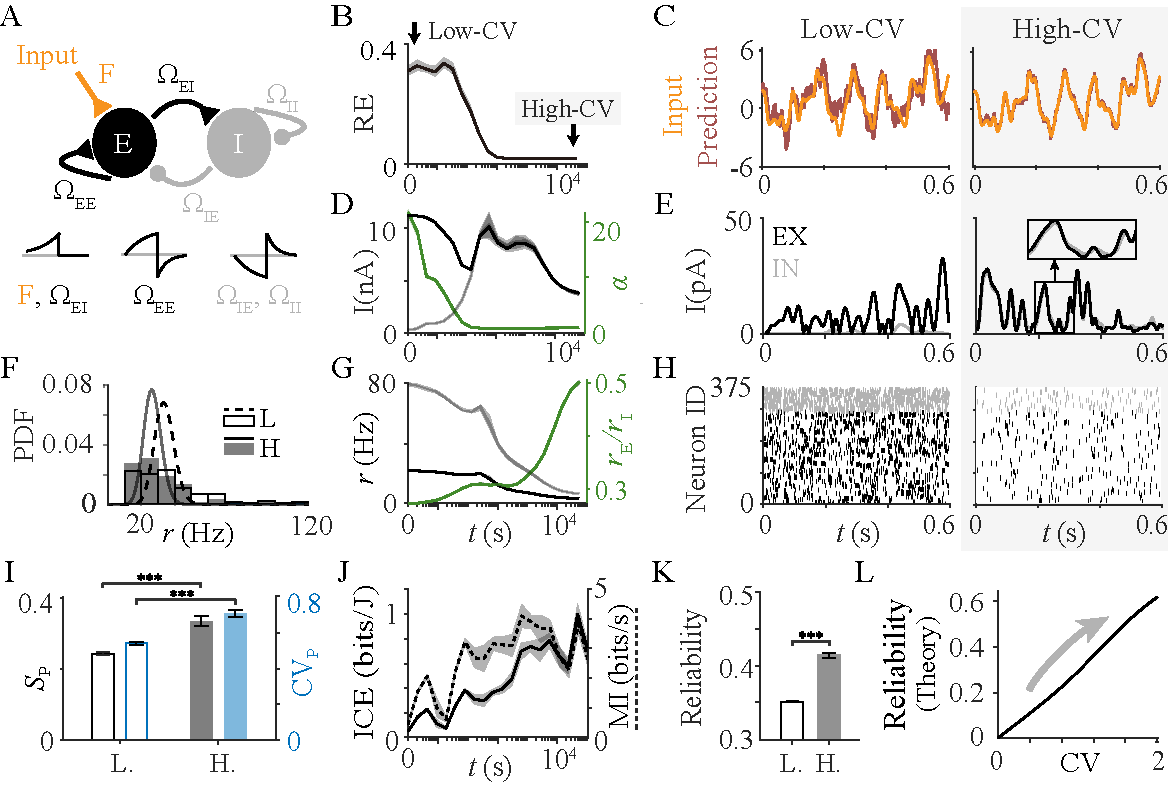
\includegraphics[scale=0.6]{figures/Figure4.pdf}
\caption{\textbf{E-I balance optimizes spike-based coding in recurrent networks.}
(\textbf{A}) Network schematic: 300 E and 75 I neurons with plastic recurrent connections ($F, \Omega_{EE}, \Omega_{EI}, \Omega_{IE}, \Omega_{II}$); plasticity rules below.
(\textbf{B}) Reconstruction error (RE) decreases during learning, transitioning from a low-CV to a high-CV regime.
(\textbf{C}) Input signal (orange) and network prediction (red) in low-CV (left) and high-CV (right) states.
(\textbf{D}) Total current magnitude $I$ (black) and scaling parameter $\alpha$ (green, right axis) during learning.
(\textbf{E}) Excitatory (black, EX) and inhibitory (gray, IN) currents for low-CV (left) and high-CV (right); high-CV inset highlights E-I cancellation.
(\textbf{F}) Firing-rate distribution: broad in low-CV (L, dashed) vs.\ heavy-tailed in high-CV (H, solid).
(\textbf{G}) Mean firing rate $r$ (black) and E/I rate ratio $r_E/r_I$ (green) over time.
(\textbf{H}) Raster plots: synchronous spiking (left, low-CV) transitioning to asynchronous (right, high-CV).
(\textbf{I}) Population sparseness $S_P$ (left axis) and population CV $\mathrm{CV}_P$ (blue, right axis) for low-CV (L) vs.\ high-CV (H) states; both rise after learning ($^{***}$).
(\textbf{J}) ICE (bits/J, solid) and mutual-information rate (MI, bits/s, dashed) over training.
(\textbf{K}) Trial-to-trial spike-count agreement $P_{\mathrm{agree}}$ for L vs.\ H ($^{***}$); panel-K label ``Reliability'' is shorthand for this count-consistency metric (not decoder-based reliability).
(\textbf{L}) Theoretical $P_{\mathrm{agree}}$ vs.\ CV under Poisson-like count statistics (arrow: increasing direction); panel label ``Reliability (Theory)''.  Caveats on the restricted-reliability interpretation are in the main text.}
\label{fig:network}
\end{figure*}
